Before the training or inference processes can take place a feature selection should be performed. For the chosen grid of size $7 \times 7$ there are all together 196 features available. Out of these features only such a set of features should be chosen which carry meaningful information that will allow differentiation of objects by shape. Performing segmentation with too many features is not only more time-consuming, but also less accurate. One of the most popular and simplest algorithms for for finding an optimal set of features is a stepwise regression, which was implemented in the thesis. This is a greedy algorithm that creates a resulting set of features step by step. This method can involve only forward steps, only backward steps, or a combination of those two. Forward selection starts by an empty set of features. The first step is to choose such a feature from the whole feature set, that will give the highest precision of segmentation for a validation set. Then, in each iteration a new best feature is added to the set of already chosen features. 
\begin{figure}[ht]
    \centering
    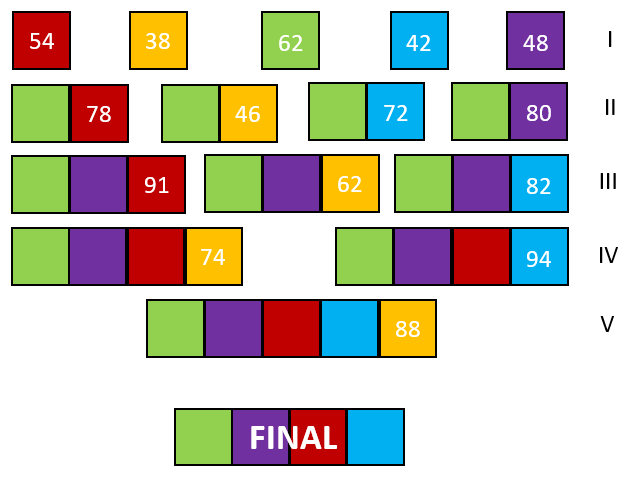
\includegraphics[width=0.60\textwidth]{images/nonlinear_intro/greedy_forward.png}
    \caption{Greedy forward feature selection}
    \label{fig:greedy_selection}
\end{figure}
Figure \ref{fig:greedy_selection} presents an example of how this method is applied for feature selection from a set of five available features each depicted as a separate coloured block. Numbers in those blocks represent the accuracy of segmentation for a set of features under consideration. As the process of feature selection is applied only to choose features for unary component of energy, there is no need to perform a full inference process to check the accuracy of segmentation. Instead, it is enough to choose the most probable label for each superpixel basing on the computation of unary potential and compare the final labelling to the ground truth. This is the measure that was used to choose the best feature in the current step. Hence, in the first iteration for all sets containing only one element this procedure is performed and the feature with highest precision is added to the final set. Then, to this feature every other feature is added forming sets of two elements and again, accuracy of segmentation for each set is measured. This procedure continues iteratively until no more features are left, or until a situation in which adding of any other feature results in worsening of the model performance. 
Backward feature selection is a very similar process, however, instead of adding new features to the set under consideration, feature elimination is performed. The procedure starts with a full set of available features. Then iteratively the worst feature is removed from this set until further elimination results in poorer accuracy of segmentation. Another possibility is to join those two methods, and make some steps forward and then some steps backward.

For this experiment feature selection was performed by a stepwise regression algorithm with five steps forward and three steps backward. From 196 available features a set of 16 features was chosen. The optimal set is combination of features representing colours of superpixels from the the already defined grid as well as percentage of red, green and blue superpixels in the neighbourhood of a given grid point. Figures \ref{fig:nonlinear_noise_free_features_colour} and \ref{fig:nonlinear_noise_free_features_percentage} present visualisations of which features were chosen by the selection algorithm.
\begin{figure}
    \centering
    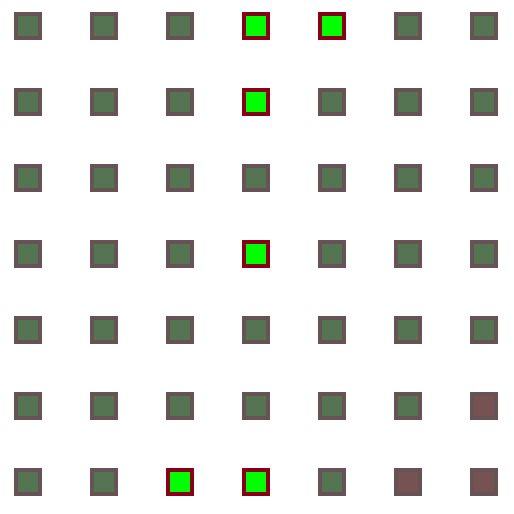
\includegraphics[width=0.5\textwidth]{nonlinear_noise_free/features/grid_colour_chosen.png}
    \caption{Chosen grid colour features for experiments on noise-free data}
    \label{fig:nonlinear_noise_free_features_colour}
\end{figure}
\begin{figure}
    \centering
    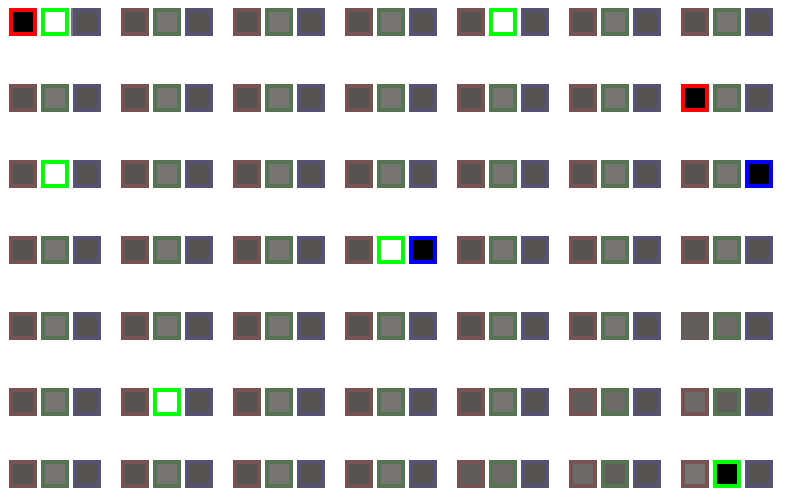
\includegraphics[width=\textwidth]{nonlinear_noise_free/features/grid_colour_percentage_chosen.png}
    \caption{Chosen grid neighbour colour percentage features for experiments on noise-free data.}
    \label{fig:nonlinear_noise_free_features_percentage}
\end{figure}

First figure depicts neighbour colour features for a sample superpixel, and the second shows neighbour colour percentage features. The way of feature presentation is the same as in \textit{section \ref{sec:nonlinear_unary_potential}: \nameref{sec:nonlinear_unary_potential}}. Features which were not chosen are covered by an extra semitransparent layer, while those which form the final feature set are left unchanged.

Optimal features were selected based on a validation set, hence, to check whether the selection was indeed optimal an extra test was performed. For images from the testing set the conditional probability $p(y|x)$ was computed for every label and for the selected set of features. The resulting probabilities are presented in figure \ref{fig:noise_free_fi1}.
In the first row an original image is depicted and the next four rows show calculated conditional probabilities, one per each label. A colour of the superpixel represents a probability that this superpixel will be assigned to the given class. The more probable the label is, the more white is the superpixel. In presented images it is visible that the algorithm has no problem in assigning proper classes to green and blue regions. The difficulty of the task lies in labelling objects into classes 0 and 3, as the only difference between objects of those classes is their shape. For these classes, the resulting probability is smaller than 100\%, therefore, there are some superpixels with different shades of grey. 

The presented probabilities form a base of computation of unary potential. If for some regions, the resulting probabilities for label 0 and 3 are more or less equal, some noised classifications may occur. In such situations, a pairwise potential is needed to ensure that neighbouring pixels from the same object will be assigned to the same class.

\begin{center}
 \renewcommand{\arraystretch}{4}
    \begin{tabular}{cccc}
        \textit{test image} &
        \fcolorbox{black}{white}{\includegraphics[align=c,width= 0.22\textwidth]{nonlinear_noise_free/fi_1/1/image.png}} &
        \fcolorbox{black}{white}{\includegraphics[align=c,width= 0.22\textwidth]{nonlinear_noise_free/fi_1/2/image.png}} &
        \fcolorbox{black}{white}{\includegraphics[align=c,width= 0.22\textwidth]{nonlinear_noise_free/fi_1/3/image.png}}  \\
        \textit{label 0} &
        \fcolorbox{black}{white}{\includegraphics[align=c,width= 0.22\textwidth]{nonlinear_noise_free/fi_1/1/label_0.png}} &
        \fcolorbox{black}{white}{\includegraphics[align=c,width= 0.22\textwidth]{nonlinear_noise_free/fi_1/2/label_0.png}} &
        \fcolorbox{black}{white}{\includegraphics[align=c,width= 0.22\textwidth]{nonlinear_noise_free/fi_1/3/label_0.png}} \\
        \textit{label 1} &
        \fcolorbox{black}{white}{\includegraphics[align=c,width= 0.22\textwidth]{nonlinear_noise_free/fi_1/1/label_1.png}} &
        \fcolorbox{black}{white}{\includegraphics[align=c,width= 0.22\textwidth]{nonlinear_noise_free/fi_1/2/label_1.png}} &
        \fcolorbox{black}{white}{\includegraphics[align=c,width= 0.22\textwidth]{nonlinear_noise_free/fi_1/3/label_1.png}} \\
        \textit{label 2} &
        \fcolorbox{black}{white}{\includegraphics[align=c,width= 0.22\textwidth]{nonlinear_noise_free/fi_1/1/label_2.png}} &
        \fcolorbox{black}{white}{\includegraphics[align=c,width= 0.22\textwidth]{nonlinear_noise_free/fi_1/2/label_2.png}} &
        \fcolorbox{black}{white}{\includegraphics[align=c,width= 0.22\textwidth]{nonlinear_noise_free/fi_1/3/label_2.png}} \\
        \textit{label 3} &
        \fcolorbox{black}{white}{\includegraphics[align=c,width= 0.22\textwidth]{nonlinear_noise_free/fi_1/1/label_3.png}} &
        \fcolorbox{black}{white}{\includegraphics[align=c,width= 0.22\textwidth]{nonlinear_noise_free/fi_1/2/label_3.png}} &
        \fcolorbox{black}{white}{\includegraphics[align=c,width= 0.22\textwidth]{nonlinear_noise_free/fi_1/3/label_3.png}}
    \end{tabular}
    \captionof{figure}{Visual representation of conditional probabilities $p(y|x)$ for three sample noise-free images.}
    \label{fig:noise_free_fi1}
\end{center}
